\documentclass[17pt]{extarticle}
\usepackage[T1]{fontenc}
\usepackage[utf8]{inputenc}

\usepackage{amsfonts, amsmath, amssymb}
\usepackage{mathtools}

\usepackage{geometry}
 \geometry{
 a4paper,
 landscape,
 left=3mm,
 right = 3mm,
 top=3mm,
 bottom=3mm,
 }

\usepackage{graphicx}
\usepackage{subfig}

\pagenumbering{gobble}
\usepackage{url}
%%  Defines the command \url{} that can be used to typeset url:s
%%  in text

\usepackage[parfill]{parskip}
\usepackage{ragged2e}
\usepackage{mathptmx}
\usepackage{anyfontsize}
\usepackage{t1enc}

\newcommand*{\pd}[2]{\ensuremath{\dfrac{\partial #1}{\partial #2}}}
\newcommand*{\inpd}[2]{\ensuremath{\frac{\partial #1}{\partial #2}}}
\DeclarePairedDelimiter\floor{\lfloor}{\rfloor}

\setcounter{tocdepth}{4}
\setcounter{secnumdepth}{4}

\begin{document}



\begin{center}
{\fontsize{70}{20}\selectfont github.com/nikitazozoulenko}
\end{center}
\begin{figure}
\begin{minipage}{.5\textwidth}
  	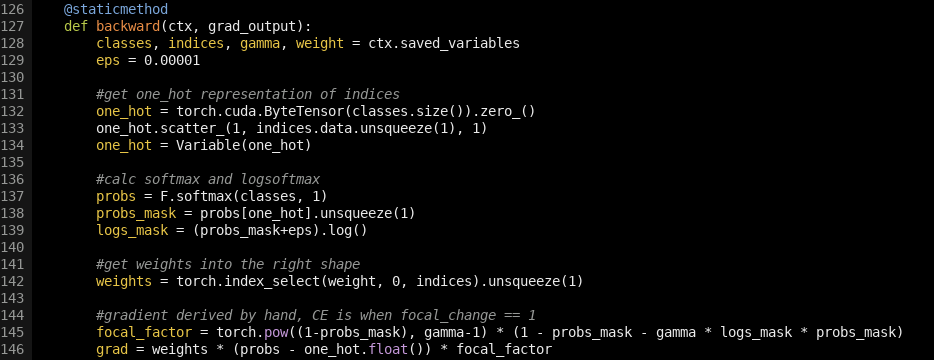
\includegraphics[scale=0.88]{focalback.png}
\end{minipage}
\end{figure}

\begin{figure}
\begin{minipage}{.5\textwidth}
  	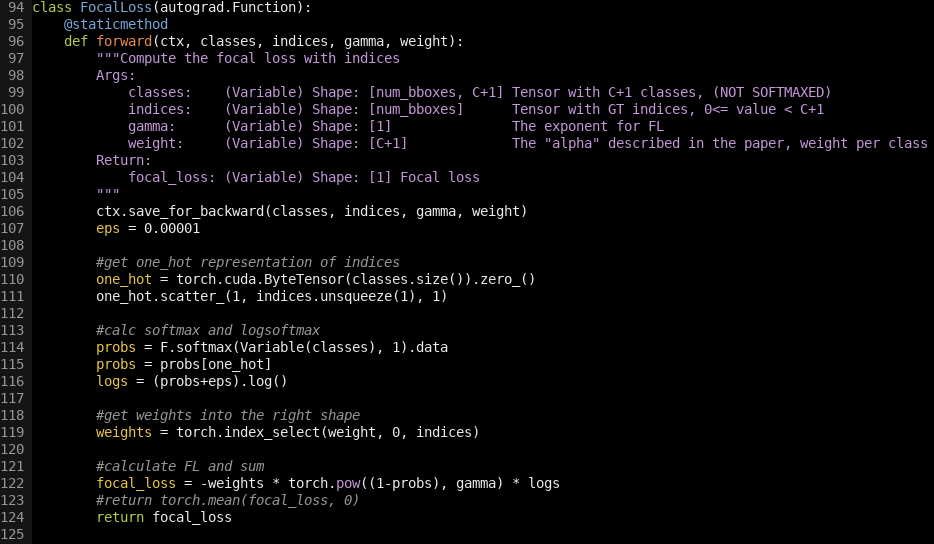
\includegraphics[scale=0.88]{focalforward.png}
\end{minipage}
\end{figure}

\end{document}


